\documentclass[../main.tex]{subfiles}
\begin{document}
	This section will give an overview of the whole system. It will be explained in its context to show how the system interacts with other systems and introduce the basic functionality of it. It will also describe what type of stakeholders will use the system and what functionality  is available for each type. At last, the constraints and the assumptions for the system will be presented.
	\section{Product perspective}
		The system will consist only of a web portal, used to manage the practices and informations about them. It will used also to managing practices by logged users.\\
		The application needs to store and retrieve data from a database. The data will presented to users via web portal.
		\begin{figure}[h]
			\centering
			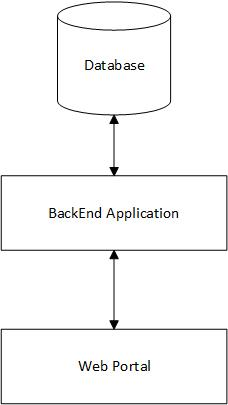
\includegraphics[width=0.3\textwidth]{Disegno1}
			\caption{Block diagram}
		\end{figure}
	\section{Product functions}
		With this application, the employees will able to view and work on their own practices, while the administrators will able to retrieve all practices and managing them.\\
		The application also provides to send emails to practices' owners when they are on due date and aren't already closed.\\
		The employees can interact with their own practices to update with new activities, add information and comments and resolve them.\\
		The administrators can view all the practices to add comment for information, view all the activities done and close if resolved.\\
		The administrators can also manage other users (administrators and employees).
	\section{Constraints}
		The application is constrained by an Internet connection, due to the database used to fetch data. Both the application and the database must be hosted on-line. 
	\section{Assumptions and dependencies}
		One assumption about the product is that it can be used via desktop or mobile interface.\\
		Another assumption is that the administrators are registered during installation of the application.
\end{document}